\documentclass[]{elsarticle} %review=doublespace preprint=single 5p=2 column
%%% Begin My package additions %%%%%%%%%%%%%%%%%%%
\usepackage[hyphens]{url}

  \journal{An awesome journal} % Sets Journal name


\usepackage{lineno} % add
  \linenumbers % turns line numbering on
\providecommand{\tightlist}{%
  \setlength{\itemsep}{0pt}\setlength{\parskip}{0pt}}

\usepackage{graphicx}
\usepackage{booktabs} % book-quality tables
%%%%%%%%%%%%%%%% end my additions to header

\usepackage[T1]{fontenc}
\usepackage{lmodern}
\usepackage{amssymb,amsmath}
\usepackage{ifxetex,ifluatex}
\usepackage{fixltx2e} % provides \textsubscript
% use upquote if available, for straight quotes in verbatim environments
\IfFileExists{upquote.sty}{\usepackage{upquote}}{}
\ifnum 0\ifxetex 1\fi\ifluatex 1\fi=0 % if pdftex
  \usepackage[utf8]{inputenc}
\else % if luatex or xelatex
  \usepackage{fontspec}
  \ifxetex
    \usepackage{xltxtra,xunicode}
  \fi
  \defaultfontfeatures{Mapping=tex-text,Scale=MatchLowercase}
  \newcommand{\euro}{€}
\fi
% use microtype if available
\IfFileExists{microtype.sty}{\usepackage{microtype}}{}
\bibliographystyle{elsarticle-harv}
\usepackage{longtable}
\ifxetex
  \usepackage[setpagesize=false, % page size defined by xetex
              unicode=false, % unicode breaks when used with xetex
              xetex]{hyperref}
\else
  \usepackage[unicode=true]{hyperref}
\fi
\hypersetup{breaklinks=true,
            bookmarks=true,
            pdfauthor={},
            pdftitle={A comparison of design-based and model-based approaches for spatial data.},
            colorlinks=false,
            urlcolor=blue,
            linkcolor=magenta,
            pdfborder={0 0 0}}
\urlstyle{same}  % don't use monospace font for urls

\setcounter{secnumdepth}{5}
% Pandoc toggle for numbering sections (defaults to be off)

% Pandoc citation processing
\newlength{\cslhangindent}
\setlength{\cslhangindent}{1.5em}
\newlength{\csllabelwidth}
\setlength{\csllabelwidth}{3em}
% for Pandoc 2.8 to 2.10.1
\newenvironment{cslreferences}%
  {}%
  {\par}
% For Pandoc 2.11+
\newenvironment{CSLReferences}[2] % #1 hanging-ident, #2 entry spacing
 {% don't indent paragraphs
  \setlength{\parindent}{0pt}
  % turn on hanging indent if param 1 is 1
  \ifodd #1 \everypar{\setlength{\hangindent}{\cslhangindent}}\ignorespaces\fi
  % set entry spacing
  \ifnum #2 > 0
  \setlength{\parskip}{#2\baselineskip}
  \fi
 }%
 {}
\usepackage{calc}
\newcommand{\CSLBlock}[1]{#1\hfill\break}
\newcommand{\CSLLeftMargin}[1]{\parbox[t]{\csllabelwidth}{#1}}
\newcommand{\CSLRightInline}[1]{\parbox[t]{\linewidth - \csllabelwidth}{#1}\break}
\newcommand{\CSLIndent}[1]{\hspace{\cslhangindent}#1}

% Pandoc header

\usepackage{bm} \usepackage{bbm} \usepackage{color} \DeclareMathOperator{\var}{{var}} \DeclareMathOperator{\cov}{{cov}}

\begin{document}
\begin{frontmatter}

  \title{A comparison of design-based and model-based approaches for
spatial data.}
    \author[USEPA]{In alphabetical order Michael Dumelle\corref{1}}
   \ead{Dumelle.Michael@epa.gov} 
    \author[STLAW]{Matt Higham\corref{1}}
   \ead{mhigham@stlaw.edu} 
    \author[OSU]{Lisa Madsen}
  
    \author[USEPA]{Anthony R. Olsen}
  
    \author[NOAA]{Jay M. Ver Hoef}
  
      \address[USEPA]{United States Environmental Protection Agency, 200
SW 35th St, Corvallis, Oregon, 97333}
    \address[STLAW]{Saint Lawrence University Department of Mathematics,
Computer Science, and Statistics, 23 Romoda Drive, Canton, New York,
13617}
    \address[OSU]{Oregon State University Department of Statistics, 239
Weniger Hall, Corvallis, Oregon, 97331}
    \address[NOAA]{Marine Mammal Laboratory, Alaska Fisheries Science
Center, National Oceanic and Atmospheric Administration, Seattle,
Washington, 98115}
      \cortext[1]{Corresponding Author}
  
  \begin{abstract}
  This is the abstract.
  \end{abstract}
  
 \end{frontmatter}

\emph{Text based on elsarticle sample manuscript, see
\url{http://www.elsevier.com/author-schemas/latex-instructions\#elsarticle}}

Potential Journals:

\begin{itemize}
\tightlist
\item
  Ecological Applications
\item
  Methods in Ecology and Evolution
\item
  Journal of Applied Ecology
\item
  Environmetrics
\item
  Environmental and Ecological Statistics
\end{itemize}

\hypertarget{sec:introduction}{%
\section{Introduction}\label{sec:introduction}}

There are two general approaches for using data to make statistical
inferences about a population: design-based approaches and model-based
approaches. When data cannot be obtained for all units in a population
(population units), data on a subset of the population units is
collected in a sample. In the design-based approach, inferences about
the underlying population are informed from a probabilistic process in
which population units are selected to be in the sample. Alternatively,
in the model-based approach, inferences are made from specific
assumptions about the underlying process that generated the data. Each
paradigm has a deep historical context (Sterba, 2009) and its own set of
general advantages (Hansen et al., 1983).

\textbf{Tony O.}: Should this paragraph address that spatial information
can be incorporated in the design stage or in the analysis stage (or
both). In general, it's not clear whether we are referring to site
selection process or the estimation process

Though the design-based and model-based approaches apply to statistical
inference in a broad sense, we focus on comparing these approaches for
spatial data. We define spatial data as data that incorporates the
specific locations of the population units into either the design or
estimation process. De Gruijter and Ter Braak (1990) give an early
comparison of design-based and model-based approaches for spatial data,
quashing the belief that design-based approaches could not be used for
spatially correlated data. Thereafter, several comparisons between
design-based and model-based for spatial data have been considered, but
they tend to compare design-based approaches that ignore spatial
locations to model-based approaches (Brus and De Gruijter, 1997; Ver
Hoef, 2002; Ver Hoef, 2008). Cooper (2006) review the two approaches in
an ecological context before introducing a ``model-assisted'' variance
estimator that combines aspects from each approach. In addition to
Cooper (2006), there has been substantial research and development into
estimators that use both design and model-based principles (see e.g.
Cicchitelli and Montanari (2012), Chan-Golston et al. (2020) for a
Bayesian approach, and Sterba (2009)). More recent overviews include
Brus (2020) and Wang et al. (2012), but no numerical comparison has been
made between design-based approaches that incorporate spatial locations
and model-based approaches.

\textbf{Lisa M.}: Add paragraph describing contribution of manuscript.

The rest of this paper is organized as follows. In Section
\ref{sec:background}, we compare sampling and estimation procedures
between the design-based approach and the model-based approach. In
Section \ref{sec:numstudy}, we use simulated and real data to study the
the behavior of both approaches. And in Section \ref{sec:discussion}, we
end with a discussion and provide directions for future research.

\hypertarget{sec:background}{%
\section{Background}\label{sec:background}}

The design-based and model-based approaches incorporate randomness in
fundamentally different ways. In this section, we describe the role of
randomness and its effects on subsequent inferences. We then discuss
specific inference methods for the design-based and model-based
approaches for spatial data.

\hypertarget{comparing-design-based-vs.-model-based}{%
\subsection{Comparing Design-Based
vs.~Model-Based}\label{comparing-design-based-vs.-model-based}}

The design-based approach assumes the population is fixed. Randomness is
incorporated in the selection of population units according to a
sampling design. A sampling design assigns a positive probability of
inclusion in the sample (inclusion probability) to each population unit.
Some examples of commonly used sampling designs include simple random
sampling, stratified random sample, and cluster sampling, which we refer
to as Independent Random Sampling (IRS) survey designs. The goal is to
use the sampling design and the sampled data to estimate population
parameters like means and totals. These population parameters are
traditionally assumed to be fixed but unknown.

Treating the data as fixed and incorporating randomness through the
sampling design (top row of Figure \ref{fig:fig1} ((cite Brus 2021 here
since our figure is similar?))) yields estimators having very few other
assumptions. Confidence intervals for these types of estimators are
typically derived using limiting arguments. Means and totals, for
example, are asymptotically normally distributed by the Central Limit
Theorem. If we repeatedly sample the surface, then 95\% of all 95\%
confidence intervals constructed from a procedure with appropriate
coverage will contain the true, fixed mean. Särndal et al. (2003) and
Lohr (2009) provide thorough reviews of the design-based approach.

\textbf{Jay VH}: I think it is important to stress that the limiting
distribution is over all possible randomizations, constrained by
whatever design is used.

\textbf{Jay VH}: quantity is vague. We should stick with variables, or
realized variables (we might also call these values, but we should
define and establish a consistent terminology early on.) \textbf{Matt
H}: I think, though this comment is for this paragraph, we should
establish the terminology earlier.

The model-based approach assumes the data are a random realization of a
data-generating process. Randomness is often incorporated through
distributional assumptions on this process and need not be incorporated
through random sampling (bottom row of Figure \ref{fig:fig1}). Instead
of estimating fixed but unknown parameters (as in the design-based
approach), the goal of model-based inference in the spatial context is
often \emph{prediction} of an unknown quantity. For example, suppose the
realized mean of all population units is the quantity of interest.
Instead of \emph{estimating} a fixed unknown mean, we are
\emph{predicting} the value of the mean, a random variable. We know that
if we sampled all population units, we would have an exact prediction
for the mean of our one realized process, without any uncertainty.

Assuming the data is a realization of a specific data-generating process
yields predictors that are linked to distributional assumptions. These
distributional assumptions are used to derive prediction intervals. The
distributional assumptions allow the prediction intervals to be more
precise. If we repeatedly generate the response values from a fixed
spatial process and obtain a sample, then 95\% of all 95\% prediction
intervals constructed from a procedure with appropriate coverage will
contain their respective realized means. Cressie (1993) and
Schabenberger and Gotway (2017) provide reviews of model-based
approaches for spatial data.

\begin{figure}
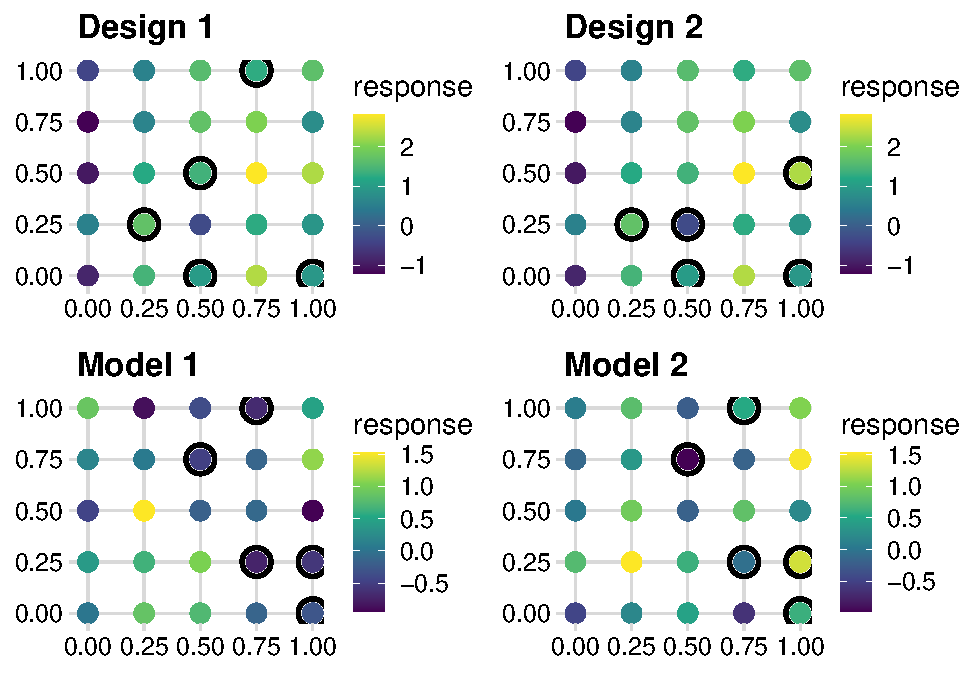
\includegraphics[width=1\linewidth]{SpatialDVM_Manuscript_files/figure-latex/fig1-1} \caption{A comparison of sampling under the design-based and model-based frameworks. Points circled are those that are sampled. In the top row, we have one fixed population, and three random samples of n = 4. The response values at each site are fixed, but we obtain different estimates for the mean response because the randomly sampled sites vary from sample to sample. In the bottom row, we have three realizations of the same spatial process sampled at the same locations. The spatial process generating the response values has a single mean, but the realized mean is different in each of the three panels.}\label{fig:fig1}
\end{figure}

\textbf{Tony O.}: Before this section is it useful to have a section
that lays out the general site selection and general analysis options.
Thinking about site selection as design-based IRS, design-based GRTS,
Arbitrary set of sites, selection for model-based. Then general analysis
options as design-based no spatial, design-based spatial, model-based.
This four by three table would show that model-based analyses are
possible for all selection options. Design-based options with no spatial
info possible for IRS-based and GRTS-based. Design-based options with
spatial info possible for GRTS-based.

\textbf{Jay VH}: What about the design for model-based inference?
Strictly speaking, it is fixed -- there is no probabilistic use of a
randomized design. However, we are going to have to deal with Diggle et
al.~(2010).

\hypertarget{spatially-balanced-design-and-analysis}{%
\subsection{Spatially Balanced Design and
Analysis}\label{spatially-balanced-design-and-analysis}}

\textbf{Lisa M.}: Need a more precise definition of ``miniature'' in
this context, and need an example.

\textbf{Jay VH}: Saying ``the distribution of the sampled population
units mirrors the density of\ldots{}'' is confusing to me. Are these
formal statistical definitions of distribution (cumulative distribution
function) and density (probability density function)? Wouldn't IRS
sample be a miniature, as it should, on average, mirror a population?

The design-based approach can use spatial locations to obtain spatially
balanced samples. First we discuss spatial balance with respect to the
population (Stevens and Olsen, 2004). A sample is spatially balanced
with respect to the population if the sampled population units are a
miniature of the population units. A sample is a miniature of the
population if the distribution of the sampled population units mirrors
the density of all population units. Spatial balance with respect to the
population is different than spatial balance with respect to geography.
A sample that is spatially balanced with respect to geography is spread
out in some type of equidistant manner over geographical space and is
not meant to be miniatures of the population. When we refer to spatial
balance henceforth, we mean spatial balance with respect to the
population.

Spatially balanced samples are useful because they tend to yield
estimates that have lower variance than estimates constructed from
sampling designs lacking spatial balance (Barabesi and Franceschi, 2011;
Benedetti et al., 2017; Grafström and Lundström, 2013; Robertson et al.,
2013; Stevens and Olsen, 2004; Wang et al., 2013). To quantify spatial
balance, Stevens and Olsen (2004) proposed loss functions based on
Voroni polygons. The first spatially balanced sampling algorithm that
saw widespread use was the Generalized Random Tessellation Stratified
(Stevens and Olsen, 2004). Since GRTS was developed, several other
spatially balanced sampling algorithms have emerged, including the Local
Pivotal Method (Grafström et al., 2012; Grafström and Matei, 2018),
Spatially Correlated Poisson Sampling (Grafström, 2012), Balanced
Acceptance Sampling (Robertson et al., 2013), Within-Sample-Distance
(Benedetti and Piersimoni, 2017), and Halton Iterative Partitioning
(Robertson et al., 2018). We focus on the Generalized Random
Tessellation Stratified (GRTS) algorithm to select spatially balanced
sampling because it has several attractive properties, including
\textbf{Lisa M.}: List major attractive properties, and detailed by
Stevens and Olsen (2004) and Dumelle et al. (2021).

The GRTS algorithm is used to sample from finite and infinite
populations and works by utilizing a mapping between two-dimensional and
one-dimensional space. The population units in two-dimensional space are
divided into cells using a hierarchical index. Population units are then
mapped to a one-dimensional line via the hierarchical indexing. The line
length of each population unit equals its inclusion probability. A
systematic sample is conducted on the line and these samples are linked
to a population unit in two-dimensional space, which results in the
desired sample. Stevens and Olsen (2004) and Dumelle et al. (2021)
provide further details.

After collecting a sample using the GRTS algorithm, the data are used to
estimate population parameters. The Horvitz-Thompson estimator (Horvitz
and Thompson, 1952) yields unbiased estimates of population means and
totals. For example, if \(\tau\) is a population total, then the
Horvitz-Thompson estimator of \(\tau\) (denoted by \(\hat{\tau}_{ht}\)),
is given by \begin{align}\label{eq:ht}
  \hat{\tau}_{ht} = \sum_{i = 1}^n Z_i \pi_i^{-1},
\end{align} where \(Z_i\) and \(\pi_i\) are the observed value and
inclusion probability of the \(i\)th population unit selected in the
sample. A similar formula exists for estimating the mean, \(\mu\).
Horvitz and Thompson (1952) and Sen (1953) provide variance estimators
for \(\hat{\tau}_{ht}\), but they have two drawbacks. First, they rely
on calculating \(\pi_{ij}\), the probability that population unit \(i\)
and population unit \(j\) are included in the sample, and this can be
very difficult to calculate. Second, they ignore the spatial locations
of the population units. To address these drawbacks, Stevens and Olsen
(2003) proposed a local neighborhood variance estimator. The local
neighborhood variance estimator does not rely on \(\pi_{ij}\), and it
incorporates spatial locations by assigning higher weights to nearby
observations. Stevens and Olsen (2003) show this variance estimators
tends to reduce the estimated standard error of \(\hat{\tau}\), yielding
narrower confidence confidence intervals for \(\tau\).

\hypertarget{finite-population-block-kriging}{%
\subsection{Finite Population Block
Kriging}\label{finite-population-block-kriging}}

Finite Population Block Kriging (FPBK) is a model-based approach that
expands the geostatistical Kriging framework to the finite population
setting (Ver Hoef, 2008). Instead of basing inference off of a specific
sampling design, we assume the data are generated by a spatial process.
Ver Hoef (2008) gives details on the theory of FPBK, but some of the
basic principles are summarized below. Let
\(\mathbf{z} \equiv \{\text{z}(s_1), \text{z}(s_2), . . . , \text{z}(s_N) \}\)
be a response vector at locations \(s_1\), \(s_2\), . . . , \(s_N\) that
can be measured at the \(N\) population units and is represented as an
\(N \times 1\) vector. Suppose we want to predict some linear function
of the response variable,
\(f(\mathbf{z}) = \mathbf{b}^\prime \mathbf{z}\), where
\(\mathbf{b}^\prime\) is a \(1 \times N\) vector of weights. For
example, if we want to predict the population total across all
population units, then we would use a vector of 1's for the weights.

However, we often only have a sample of the \(N\) population units.
Denoting quantities that are part of the sampled population units with a
subscript \emph{s} and quantities that are part of the unsampled
population units with a subscript \emph{u},

\begin{equation}
\begin{pmatrix} \label{equation:Zmarginal}
    \mathbf{z}_s      \\
    \mathbf{z}_u
\end{pmatrix}
=
\begin{pmatrix}
  \mathbf{X}_s    \\
  \mathbf{X}_u
\end{pmatrix}
\bm{\beta} +
\begin{pmatrix}
\bm{\delta}_s    \\
\bm{\delta}_u
\end{pmatrix},
\end{equation} where \(\mathbf{X}_s\) and \(\mathbf{X}_u\) are the
design matrices for the sampled and unsampled population units,
respectively; \(\beta\) is the parameter vector of fixed effects; and
\(\bm{\delta}_s\) and \(\bm{\delta}_u\) are random errors for the
sampled and unsampled population units, respectively. Denoting
\(\bm{\delta} \equiv [\bm{\delta}_s \,\, \bm{\delta}_u]'\), we assume
the expectation of \(\bm{\delta}\) equals \(\mathbf{0}\).

We also assume that there is spatial correlation in \(\bm{\delta}\),
which can be modeled using a covariance function. It is common to assume
the covariance function is second-order stationary and isotropic
(Cressie, 1993), and that the spatial covariance decreases as the
separation between population units increases. Many spatial covariance
functions exist, but the primary function we use throughout the
simulations and applications in this manuscript is the exponential
covariance function: the \(i,j^{th}\) entry for
\(\mathop{\mathrm{{cov}}}(\bm{\delta})\) is \mbox{}
\begin{align}\label{equation:expcov}
\mathop{\mathrm{{cov}}}(\delta_i, \delta_j) = \theta_1\exp(-3h_{i,j}/\theta_2) + \theta_3\mathbbm{1}\{\mathbf{h}_{i,j} = 0\}, 
\end{align} where \(h_{i,j}\) is the distance between population units
\(i\) and \(j\), and \(\bm{\theta}\) is a vector of spatial covariance
parameters of the partial sill \(\theta_1\), the range \(\theta_2\), and
the nugget \(\theta_3\); and, \(\mathbbm{1}\) is equal to 1 when
distance \(h_i,j\) is equal to 0, and equal to 0 otherwise. However, any
spatial covariance function could be used in the place of the
exponential, including functions that allow for non-stationarity or
anisotropy (Chiles and Delfiner, 1999, pp. 80--93).

\textbf{Lisa M.} : Include formulas. Perhaps, but, these are very heavy
in notation and matrix algebra. We might consider, however, adding the
formulas to an Appendix.

With the above model formulation, the Best Linear Unbiased Predictor
(BLUP) for \(f(\mathbf{b}'\mathbf{z})\) and its prediction variance can
be computed. While details of the derivation are in (Ver Hoef, 2008), we
note here that the predictor and its variance are both moment-based.

We note that we only use FPBK in this paper in order to focus more on
comparing the design-based and model-based approaches. However,
k-nearest-neighbors (Fix and Hodges, 1951; Ver Hoef and Temesgen, 2013),
random forest (Breiman, 2001), Bayesian models (Chan-Golston et al.,
2020), among others, can also be used to obtain predictions for a mean
or total from spatially correlated responses in a finite population
setting. We choose to use FPBK because it is faster than a Bayesian
approach and random forest and because Ver Hoef and Temesgen (2013)
showed that the method outperforms k-nearest-neighbors in many
scenarios.

\hypertarget{sec:numstudy}{%
\section{Numerical Study}\label{sec:numstudy}}

We used a numerical simulation study to investigate performance of four
design-analysis combinations, summarized in Table
\ref{tab:designanalysis}.

\begin{longtable}[]{@{}lll@{}}
\caption{\label{tab:designanalysis} Types of Sampling Design and
Analysis combinations considered in the simulation study. The columns
give the two types of sampling designs while the rows give the two types
of analyses.}\tabularnewline
\toprule
& IRS & GRTS \\
\midrule
\endfirsthead
\toprule
& IRS & GRTS \\
\midrule
\endhead
Design & IRS-Design & GRTS-Design \\
Model & IRS-Model & GRTS-Model \\
\bottomrule
\end{longtable}

We used a crossed design with the simulation parameters given in Table
\ref{tab:parmtab} for a total of 36 scenarios. All scenarios used
exponential correlation with an effective range of \(\sqrt{2}\) for
\(N = 900\) response values simulated on the unit square in either
random locations (Site Locations = Random) or gridded locations (Site
Locations = Gridded). The mean for the spatial process generating the
response was set to zero.

For the lognormal scenarios, the response values were simulated using
the specified correlation parameters using a normal distribution and
were subsequently exponentiated. A total variance of 2 and a mean of 0
on the normal scale is equivalent to a total variance of 47 and a mean
of 2.72 after exponentiation. Therefore, when the model-based methods
were used for lognormal response, the correlation was mis-specified. We
chose to simulate values with a lognormal distribution so that we could
test the model-based analysis approach with a mis-specified model and so
that we could test both analysis approaches on data that exhibits a
large amount of skewness.

\begin{longtable}[]{@{}llll@{}}
\caption{\label{tab:parmtab} Simulation parameters. Total variability
for all scenarios was 2 so that the partial sill was 0, 1, or
1.8.}\tabularnewline
\toprule
& & & \\
\midrule
\endfirsthead
\toprule
& & & \\
\midrule
\endhead
Sample Size (n) & 50 & 100 & 200 \\
Site Locations & Random & Gridded & \\
Partial Sill / Total Variance & 0 & 0.5 & 0.9 \\
Response Type & Normal & Lognormal & \\
\bottomrule
\end{longtable}

There were 2000 simulation trials for each of the 36 parameter
combinations. In each trial, response values were generated from a
spatial process with the specified parameters, and a GRTS sample and an
IRS sample were selected. For the GRTS sample, the design-based approach
using the local neighborhood variance (GRTS-Design) and a model-based
approach were applied (GRTS-Model). For the IRS sample, the design-based
approach using the simple random sample variance (IRS-Design) and a
model-based approach were applied (IRS-Model).

The GRTS algorithm and the local neighborhood variance estimator are
available in the \textbf{\textsf{R}} package \texttt{spsurvey} (Dumelle
et al., 2021). FPBK can be readily performed in \texttt{R} with the
\texttt{sptotal} package (Higham et al., 2020). We use \texttt{sptotal}
for both the simulation analysis and the application, estimating
parameters with Restricted Maximum Likelihood (REML).

Figure \ref{fig:figeff} shows the relative efficiency of the four
approaches from Table \ref{tab:designanalysis} with ``IRS-Design'' as
the baseline: \mbox{} \begin{equation*}
\text{E} = \frac{\text{rMSPE of approach}}{\text{rMSPE of IRS-Design}},
\end{equation*}

where rMSPE is the root-Mean-Squared-Prediction-Error. When there is no
spatial correlation (top row), the four approaches have approximately
equal rMSPE, even when the assumptions of the model-based approaches are
violated. So, using GRTS or using a spatial model does not result in
much loss in efficiency even if the response variable is not spatially
correlated. When there is high spatial correlation (bottom row), the
GRTS-Model approach tends to perform best, but difference in relative
efficiency between GRTS-Model and GRTS-Design is not very big. In the
lognormal, high partial sill settings (bottom-right facet), GRTS-Design
outperforms IRS-Model by a large margin, suggesting that the design
decision (whether to use IRS or GRTS) is more important than the
analysis decision (whether to analyze using model assumptions or not).

Unsurprisingly, Figure \ref{fig:figeff} also shows that, when the
assumptions for GRTS-Model are satisfied, the approach outperforms
GRTS-Design. However, even when the model that generates the data is
different than the model used to fit the data, as in the lognormal
response, the model-based approach still outperforms the design-based
approach when there is a high amount of spatial correlation.

\begin{figure}
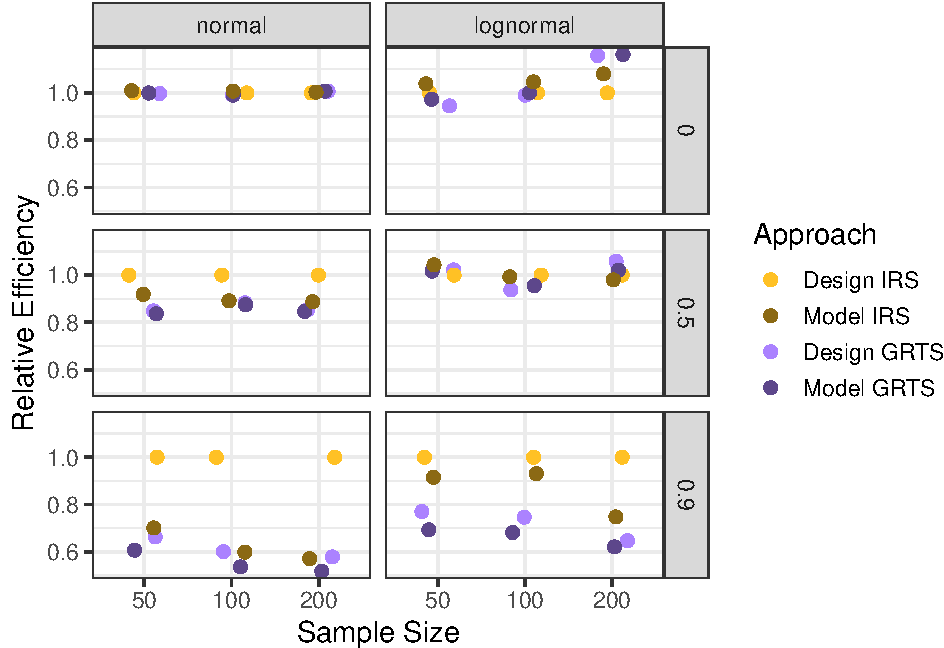
\includegraphics[width=1\linewidth]{SpatialDVM_Manuscript_files/figure-latex/figeff-1} \caption{Relative Efficiency of the four design-analysis approaches. The plot is faceted by the type of response on the columns and the partial-sill to total-variance ratio on the rows.}\label{fig:figeff}
\end{figure}

Plot Note: change colours and think about shape think about legend going
on graph

Figure \ref{fig:figconf} shows the coverage for each of the four
approaches. We see that the four approaches have somewhat similar
coverages in all settings, with GRTS-Design having slightly lower
coverage when the response is normal.

In the normal response settings, where assumptions for the model-based
approaches and the design-based approaches are satisfied, all approaches
have coverage around the nominal 0.95. Because the intervals are
symmetric, normal-based intervals, the coverages are generally lower
than the nominal 95\%. We see that, because the sampling distribution of
the mean is asymptotically normal (reference for this? a spatial version
of CLT), the coverages when the sample size is 200 are much closer to
the nominal 95\% than the coverages when the sample size is 50. In
general, the more skewed the distribution of the response, the larger
the sample size needed to ensure proper coverage of these normal-based
intervals.

Do we want to mention stuff like what's in these next bullet points or
no?

\begin{itemize}
\tightlist
\item
  for the model-based approach, the more skewed the population is, the
  higher the sample size needed to satisfy CLT for predicting a mean.
  The derivation of the BLUP is entirely moment-based (no distribution
  assumed) but we still need to assume a distribution to estimate
  spatial parameters and to generate bounds of a prediction interval.
\item
  many confidence intervals generated for design-based approaches also
  rely on the CLT and the normal distribution to generate the interval.
  Again, for highly skewed data with a small sample size, this
  assumption is violated even though all of the assumptions for
  generating the estimator are valid.
\end{itemize}

\begin{figure}
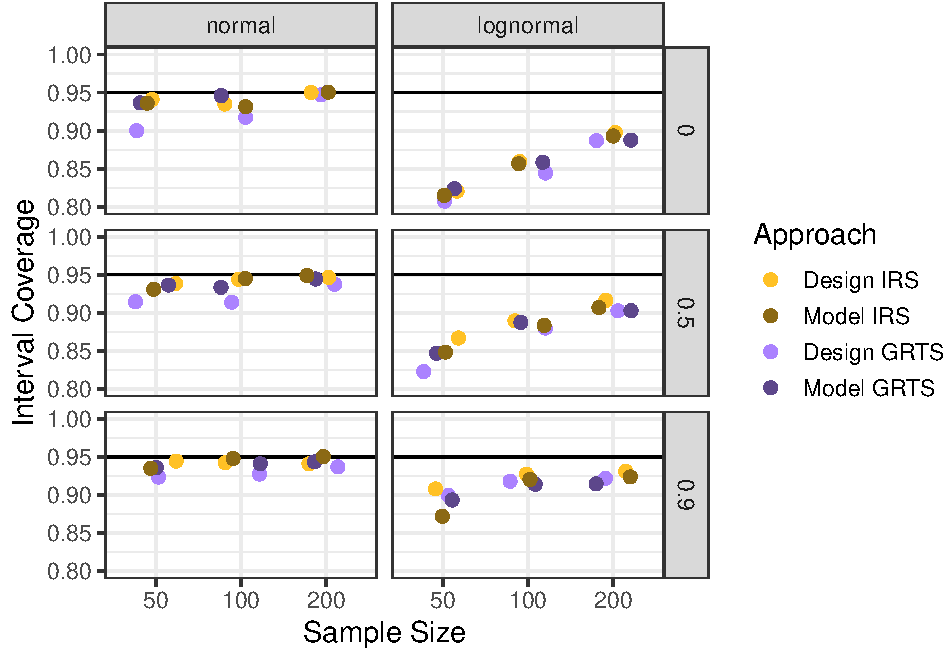
\includegraphics[width=1\linewidth]{SpatialDVM_Manuscript_files/figure-latex/figconf-1} \caption{Coverage of the four design-analysis approaches. All confidence intervals are normal-based and have a nominal confidence level of 0.95, marked with a horizontal line. The plot is faceted by the type of response on the columns and the partial-sill to total-variance ratio on the rows.}\label{fig:figconf}
\end{figure}

\hypertarget{application}{%
\section{Application}\label{application}}

The Environmental Protection Agency (EPA), states, and tribes
periodically conduct National Aquatic Research Surveys (NARS) in the
United States to assess the water quality of various bodies of water. We
will use the 2012 National Lakes Assessment (NLA), which measures
various aspects of lake health and quality in lakes in the contiguous
United States, to obtain an interval for mean mercury concentration.
Although all lakes in the survey were measured in 2012, there may not
always be enough time or money to do so. Therefore, we will explore
whether or not we can still obtain an adequately precise estimate for
the realized mean mercury concentration if we only take a sample of 100
of the 986 lakes.

\begin{figure}
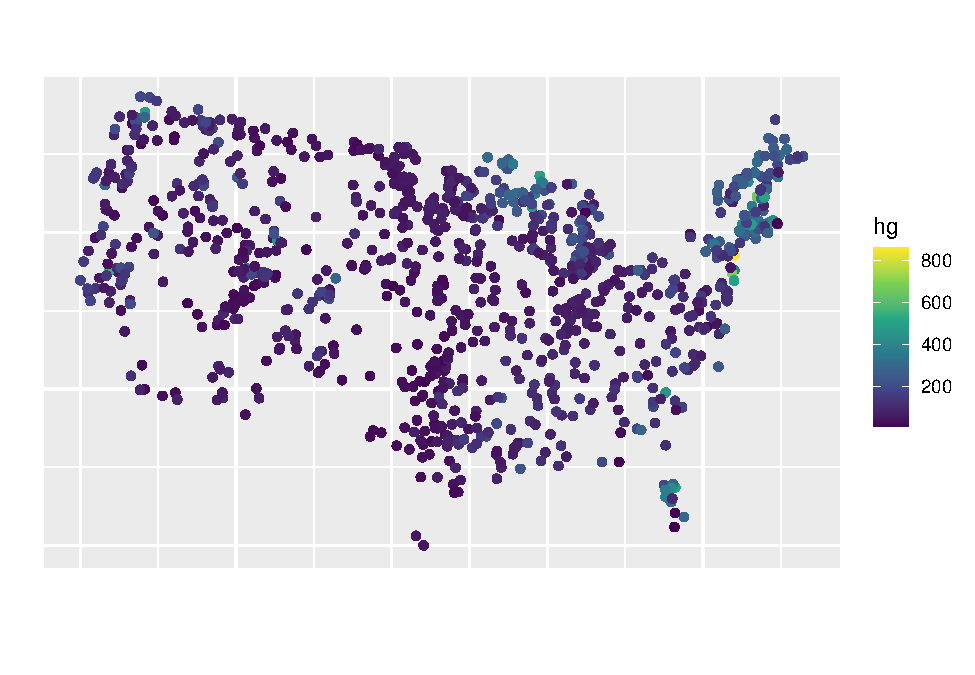
\includegraphics[width=1\linewidth]{SpatialDVM_Manuscript_files/figure-latex/figdata-1} \caption{Population distribution of mercury concentration for 986 lakes in the contiguous United States. Thirty-five lakes were dropped from the analysis because they were missing mercury concentration.}\label{fig:figdata}
\end{figure}

Figure \ref{fig:figdata} shows that mercury concentration is
right-skewed, with most lakes having a low value of mercury
concentration but a few having a much higher concentration. Mercury
concentration exhibits some spatial correlation, with high mercury
concentrations in lakes in the northeast and north central United
States. Because we are considering these lakes to be our entire
population, we know that the realized mean mercury concentration is
103.2 ng / g.

\begin{longtable}[]{@{}lrrrr@{}}
\caption{\label{tab:appliedtab} Application of design-based and
model-based approaches to the NLA data set on mercury concentration. The
true mean concentration is 103.2 103.2 ng / g}\tabularnewline
\toprule
Approach & Estimate & SE & 95\% LB & 95\% UB \\
\midrule
\endfirsthead
\toprule
Approach & Estimate & SE & 95\% LB & 95\% UB \\
\midrule
\endhead
IRS-Design & 112.7 & 8.8 & 95.4 & 129.9 \\
IRS-Model & 110.5 & 7.9 & 95.0 & 125.9 \\
GRTS-Design & 101.8 & 6.1 & 89.8 & 113.7 \\
GRTS-Model & 102.3 & 5.9 & 90.8 & 113.9 \\
\bottomrule
\end{longtable}

Table \ref{tab:appliedtab} shows the application of a design-based
analysis on an IRS, a model-based analysis on an IRS, a design-based
analysis on a GRTS sample, and a model-based analysis on a GRTS sample.
We see that, for all four analyses, the true realized mean mercury
concentration is within the bounds of the 95\% intervals. However, we
should not generalize the results of this particular realization to any
other data set or even to other potential samples of this data set.

\pagebreak

But, we do note a couple of patterns. The design-based IRS analysis
shows the largest standard error: a likely reason is that this is the
only approach that does not use the spatial correlation in mercury
concentration across the contiguous United States. We also see that, for
the samples drawn, the both analyses with the GRTS sampling design have
a lower standard error than the analyses with the IRS sampling design.
We would expect this to be the case for most samples because mercury
concentration exhibits spatial correlation so a spatially balanced
sample should usually yield a lower standard error. If it is acceptable
to have an interval for mean mercury concentration of about 25 ng / g
and if we ignore the other variables that the EPA collects information
on in these NLA surveys, then the EPA could consider sampling just 50
lakes to save time and money.

\hypertarget{sec:discussion}{%
\section{Discussion}\label{sec:discussion}}

\begin{itemize}
\item
  Pros of Design-Based (items we are not exploring): computationally
  efficient, few assumptions, more naturally handles binary data,
\item
  Pros of Model-Based (items we are not exploring): covariate inference,
  more efficient small-area estimation, model selection?, estimated
  spatial parameters to better understand spatial structure,
  site-by-site predictions/prediction map
\end{itemize}

\hypertarget{references}{%
\section*{References}\label{references}}
\addcontentsline{toc}{section}{References}

\hypertarget{refs}{}
\begin{CSLReferences}{1}{0}
\leavevmode\hypertarget{ref-barabesi2011sampling}{}%
Barabesi, L., Franceschi, S., 2011. Sampling properties of spatial total
estimators under tessellation stratified designs. Environmetrics 22,
271--278.

\leavevmode\hypertarget{ref-benedetti2017spatially}{}%
Benedetti, R., Piersimoni, F., 2017. A spatially balanced design with
probability function proportional to the within sample distance.
Biometrical Journal 59, 1067--1084.

\leavevmode\hypertarget{ref-benedetti2017spatiallyreview}{}%
Benedetti, R., Piersimoni, F., Postiglione, P., 2017. Spatially balanced
sampling: A review and a reappraisal. International Statistical Review
85, 439--454.

\leavevmode\hypertarget{ref-breiman2001random}{}%
Breiman, L., 2001. Random forests. Machine learning 45, 5--32.

\leavevmode\hypertarget{ref-brus1997random}{}%
Brus, D., De Gruijter, J., 1997. Random sampling or geostatistical
modelling? Choosing between design-based and model-based sampling
strategies for soil (with discussion). Geoderma 80, 1--44.

\leavevmode\hypertarget{ref-brus2020statistical}{}%
Brus, D.J., 2020. Statistical approaches for spatial sample survey:
Persistent misconceptions and new developments. European Journal of Soil
Science.

\leavevmode\hypertarget{ref-chan2020bayesian}{}%
Chan-Golston, A.M., Banerjee, S., Handcock, M.S., 2020. Bayesian
inference for finite populations under spatial process settings.
Environmetrics 31, e2606.

\leavevmode\hypertarget{ref-chiles1999geostatistics}{}%
Chiles, J.-P., Delfiner, P., 1999. Geostatistics: {Modeling Spatial
Uncertainty}. {John Wiley \& Sons}, New York.

\leavevmode\hypertarget{ref-cicchitelli2012model}{}%
Cicchitelli, G., Montanari, G.E., 2012. Model-assisted estimation of a
spatial population mean. International Statistical Review 80, 111--126.

\leavevmode\hypertarget{ref-cooper2006sampling}{}%
Cooper, C., 2006. Sampling and variance estimation on continuous
domains. Environmetrics: The official journal of the International
Environmetrics Society 17, 539--553.

\leavevmode\hypertarget{ref-cressie1993statistics}{}%
Cressie, N., 1993. Statistics for spatial data. John Wiley \& Sons.

\leavevmode\hypertarget{ref-de1990model}{}%
De Gruijter, J., Ter Braak, C., 1990. Model-free estimation from spatial
samples: A reappraisal of classical sampling theory. Mathematical
geology 22, 407--415.

\leavevmode\hypertarget{ref-dumelle2021spsurvey}{}%
Dumelle, M., Olsen, A.R., Kincaid, T., Weber, M., 2021. Selecting and
analyzing spatial probability samples in r using spsurvey. Manuscript
Submitted for Publication.

\leavevmode\hypertarget{ref-fix1951discriminatory}{}%
Fix, E., Hodges, J.L., 1951. Discriminatory analysis, nonparametric
discrimination: Consistency properties. USAF School of Aviation
Medicine.

\leavevmode\hypertarget{ref-grafstrom2012spatiallypoisson}{}%
Grafström, A., 2012. Spatially correlated poisson sampling. Journal of
Statistical Planning and Inference 142, 139--147.

\leavevmode\hypertarget{ref-grafstrom2013well}{}%
Grafström, A., Lundström, N.L., 2013. Why well spread probability
samples are balanced. Open Journal of Statistics 3, 36--41.

\leavevmode\hypertarget{ref-grafstrom2012spatially}{}%
Grafström, A., Lundström, N.L., Schelin, L., 2012. Spatially balanced
sampling through the pivotal method. Biometrics 68, 514--520.

\leavevmode\hypertarget{ref-grafstrom2018spatially}{}%
Grafström, A., Matei, A., 2018. Spatially balanced sampling of
continuous populations. Scandinavian Journal of Statistics 45, 792--805.

\leavevmode\hypertarget{ref-hansen1983evaluation}{}%
Hansen, M.H., Madow, W.G., Tepping, B.J., 1983. An evaluation of
model-dependent and probability-sampling inferences in sample surveys.
Journal of the American Statistical Association 78, 776--793.

\leavevmode\hypertarget{ref-higham2020sptotal}{}%
Higham, M., Ver Hoef, J., Bryce, F., 2020. Sptotal: Predicting totals
and weighted sums from spatial data.

\leavevmode\hypertarget{ref-horvitz1952generalization}{}%
Horvitz, D.G., Thompson, D.J., 1952. A generalization of sampling
without replacement from a finite universe. Journal of the American
statistical Association 47, 663--685.

\leavevmode\hypertarget{ref-lohr2009sampling}{}%
Lohr, S.L., 2009. Sampling: Design and analysis. Nelson Education.

\leavevmode\hypertarget{ref-robertson2013bas}{}%
Robertson, B., Brown, J., McDonald, T., Jaksons, P., 2013. BAS: Balanced
acceptance sampling of natural resources. Biometrics 69, 776--784.

\leavevmode\hypertarget{ref-robertson2018halton}{}%
Robertson, B., McDonald, T., Price, C., Brown, J., 2018. Halton
iterative partitioning: Spatially balanced sampling via partitioning.
Environmental and Ecological Statistics 25, 305--323.

\leavevmode\hypertarget{ref-sarndal2003model}{}%
Särndal, C.-E., Swensson, B., Wretman, J., 2003. Model assisted survey
sampling. Springer Science \& Business Media.

\leavevmode\hypertarget{ref-schabenberger2017statistical}{}%
Schabenberger, O., Gotway, C.A., 2017. Statistical methods for spatial
data analysis. CRC press.

\leavevmode\hypertarget{ref-sen1953estimate}{}%
Sen, A.R., 1953. On the estimate of the variance in sampling with
varying probabilities. Journal of the Indian Society of Agricultural
Statistics 5, 127.

\leavevmode\hypertarget{ref-sterba2009alternative}{}%
Sterba, S.K., 2009. Alternative model-based and design-based frameworks
for inference from samples to populations: From polarization to
integration. Multivariate behavioral research 44, 711--740.

\leavevmode\hypertarget{ref-stevens2003variance}{}%
Stevens, D.L., Olsen, A.R., 2003. Variance estimation for spatially
balanced samples of environmental resources. Environmetrics 14,
593--610.

\leavevmode\hypertarget{ref-stevens2004spatially}{}%
Stevens, D.L., Olsen, A.R., 2004. Spatially balanced sampling of natural
resources. Journal of the american Statistical association 99, 262--278.

\leavevmode\hypertarget{ref-verhoef2002sampling}{}%
Ver Hoef, J., 2002. Sampling and geostatistics for spatial data.
Ecoscience 9, 152--161.

\leavevmode\hypertarget{ref-verhoef2008spatial}{}%
Ver Hoef, J.M., 2008. Spatial methods for plot-based sampling of
wildlife populations. Environmental and Ecological Statistics 15, 3--13.

\leavevmode\hypertarget{ref-ver2013comparison}{}%
Ver Hoef, J.M., Temesgen, H., 2013. A comparison of the spatial linear
model to nearest neighbor (k-NN) methods for forestry applications. PloS
one 8, e59129.

\leavevmode\hypertarget{ref-wang2013design}{}%
Wang, J.-F., Jiang, C.-S., Hu, M.-G., Cao, Z.-D., Guo, Y.-S., Li, L.-F.,
Liu, T.-J., Meng, B., 2013. Design-based spatial sampling: Theory and
implementation. Environmental modelling \& software 40, 280--288.

\leavevmode\hypertarget{ref-wang2012review}{}%
Wang, J.-F., Stein, A., Gao, B.-B., Ge, Y., 2012. A review of spatial
sampling. Spatial Statistics 2, 1--14.

\end{CSLReferences}


\end{document}
